\section{Estrutura Visual de Apoio à Auditoria}
\label{sec:aplicacao_web}

Para levar as explicações ao uso do auditor fiscal, foi desenvolvida uma aplicação web que apresenta, para cada CDA sintética, o \textit{rating}, a probabilidade estimada de pagamento e a explicação SHAP correspondente. A aplicação não executa o modelo durante a consulta: os resultados são calculados previamente e apenas lidos no momento do acesso, o que mantém o tempo de resposta baixo e isola os modelos de produção da interface.

\subsection{Arquitetura}

A Figura \ref{fig:arquitetura_app} resume a arquitetura. Em uma etapa de pré-cálculo, executada uma vez por \textit{setup}, uma amostra de 1.000 CDAs sintéticas passa pelo mesmo pré-processamento, pelo \textit{ensemble} de produção e pelas regras de pós-processamento descritos no Capítulo \ref{cap:metodologia}; para cada CDA, registram-se o \textit{rating}, a probabilidade e os valores SHAP, calculados pelo \textit{TreeExplainer} em cada um dos três modelos e combinados pela média. O resultado é gravado em arquivos tabulares, um por \textit{setup}, acompanhados de metadados como o nome das variáveis e o valor de referência do SHAP.

Uma interface de programação (API REST) lê esses arquivos e oferece quatro consultas: a lista de \textit{setups}, a lista paginada de CDAs de um \textit{setup}, a ficha de auditoria de uma CDA e um texto explicativo em linguagem natural. Esse texto é montado por padrão a partir de um modelo de frase preenchido com os principais fatores da CDA; a aplicação admite, opcionalmente, que um modelo de linguagem redija o texto a partir dos mesmos fatores. Como as entradas são sintéticas, nenhum dado de contribuinte real é enviado a esse serviço. A interface do usuário consome a API e organiza a informação nas telas descritas a seguir.

\begin{figure}[H]
    \centering
    \begin{tikzpicture}[
        font=\footnotesize,
        caixa/.style={draw, rounded corners=2pt, align=center, fill=gray!8, minimum height=1.05cm, inner sep=4pt, text width=3.9cm,
                     execute at begin node={\hyphenpenalty=10000\exhyphenpenalty=10000}},
        dado/.style={caixa, fill=white},
        restrito/.style={caixa, fill=gray!25},
        opcional/.style={caixa, fill=white, dashed},
        seta/.style={-{Stealth[length=2.2mm]}, thick},
        etapa/.style={font=\scriptsize\bfseries\scshape, anchor=west, text=gray!70!black}
    ]
        % 1. Pré-cálculo
        \node[etapa] at (0.05, 1.05) {1. Pré-cálculo (uma vez por \textit{setup})};
        \node[dado] (sint) at (2.1, 0) {\textbf{Base sintética}\\1.000 CDAs por \textit{setup}};
        \node[restrito] (prod) at (2.1, -1.75) {\textbf{Artefatos de produção}\\pré-processamento, 3 XGBoost e regras};
        \node[caixa] (pre) at (7.3, -0.875) {\textbf{Pré-cálculo}\\\textit{rating}, probabilidade e SHAP (média dos 3 modelos)};
        \node[dado] (arq) at (12.5, -0.875) {\textbf{Resultados por \textit{setup}}\\arquivos tabulares e metadados};
        \draw[seta] (sint.east) -- (pre.west |- sint.east);
        \draw[seta] (prod.east) -- (pre.west |- prod.east);
        \draw[seta] (pre) -- (arq);

        % 2. Consulta
        \node[etapa] at (0.05, -3.0) {2. Consulta};
        \node[caixa] (api) at (12.5, -4.2) {\textbf{API REST}\\\textit{setups}, lista de CDAs, ficha e texto explicativo};
        \node[caixa] (ui) at (7.3, -4.2) {\textbf{Interface web}\\lista, decisão, fatores, gráficos e ficha};
        \node[dado] (aud) at (2.1, -4.2) {\textbf{Auditor fiscal}\\consulta e revisa a CDA};
        \node[opcional] (llm) at (12.5, -6.6) {\textbf{Texto em linguagem natural}\\modelo de frase (padrão) ou modelo de linguagem (opcional)};
        \draw[seta] (arq) -- (api);
        \draw[seta] (api) -- (ui);
        \draw[seta] (ui) -- (aud);
        \draw[seta, dashed] (api) -- (llm);
    \end{tikzpicture}
    \caption[Arquitetura da aplicação de apoio à auditoria]{Arquitetura da aplicação de apoio à auditoria. Na etapa 1, executada uma única vez por \textit{setup}, as CDAs sintéticas passam pelos artefatos do modelo de produção (em cinza escuro, que permanecem no ambiente institucional), e o \textit{rating}, a probabilidade e os valores SHAP de cada CDA são gravados em arquivos. Na etapa 2, a API lê esses arquivos e a interface web os apresenta ao auditor, sem executar o modelo durante a consulta. O texto explicativo é gerado por um modelo de frase; a redação por modelo de linguagem, em tracejado, é opcional.}
    \label{fig:arquitetura_app}
\end{figure}

\subsection{Telas}

A tela inicial (Figura \ref{fig:app_lista}) lista as CDAs de cada \textit{setup}, em abas, com o \textit{rating} e a probabilidade estimada de cada uma. O auditor pode filtrar por classe, buscar uma CDA pelo número e ver a distribuição das classes na amostra.

\begin{figure}[H]
    \centering
    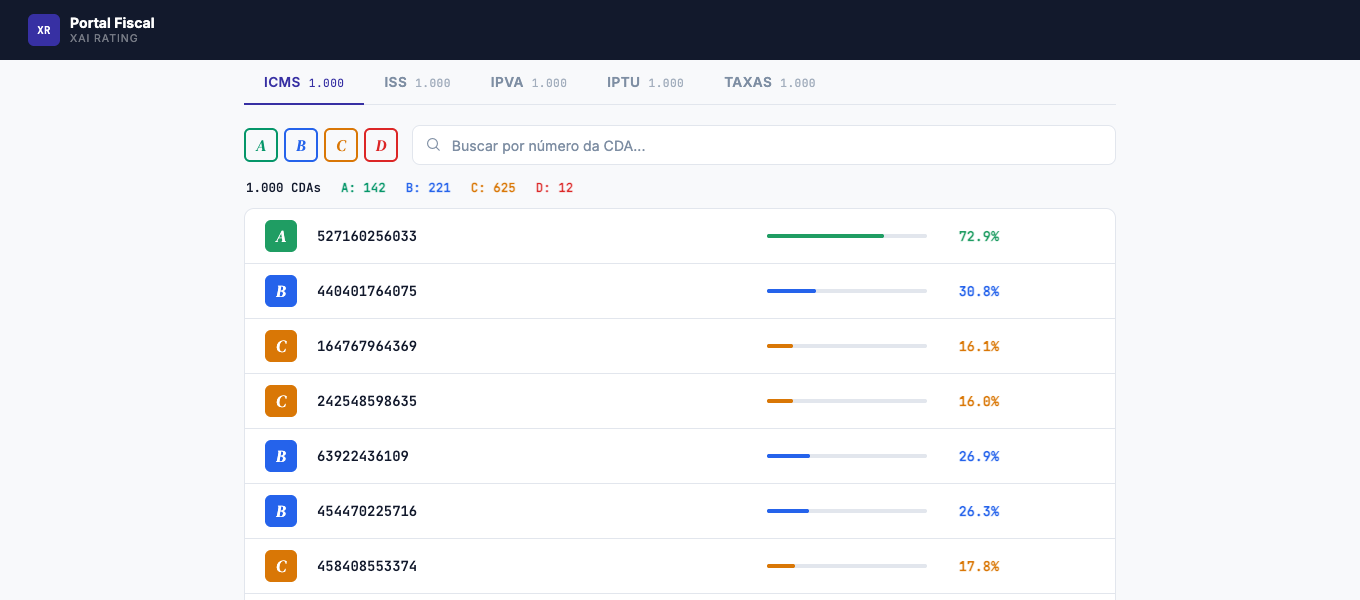
\includegraphics[width=\textwidth]{figuras/app_lista.png}
    \caption[Tela inicial da aplicação: lista de CDAs]{Tela inicial da aplicação. Cada aba corresponde a um \textit{setup}; os botões A a D filtram por classe, e o campo de busca localiza uma CDA pelo número. Cada linha mostra o \textit{rating}, o número da CDA sintética e a probabilidade estimada de pagamento. Captura de tela produzida pelos autores.}
    \label{fig:app_lista}
\end{figure}

Ao selecionar uma CDA, abre-se a ficha de auditoria. Sua parte superior (Figura \ref{fig:app_decisao}) mostra a decisão do modelo: a classe, a probabilidade, a posição da CDA em relação às demais do mesmo \textit{setup} e um texto que resume os fatores que mais elevaram e mais reduziram a chance estimada de pagamento. Logo abaixo, os cinco fatores favoráveis e os cinco desfavoráveis são listados com sua contribuição SHAP.

\begin{figure}[H]
    \centering
    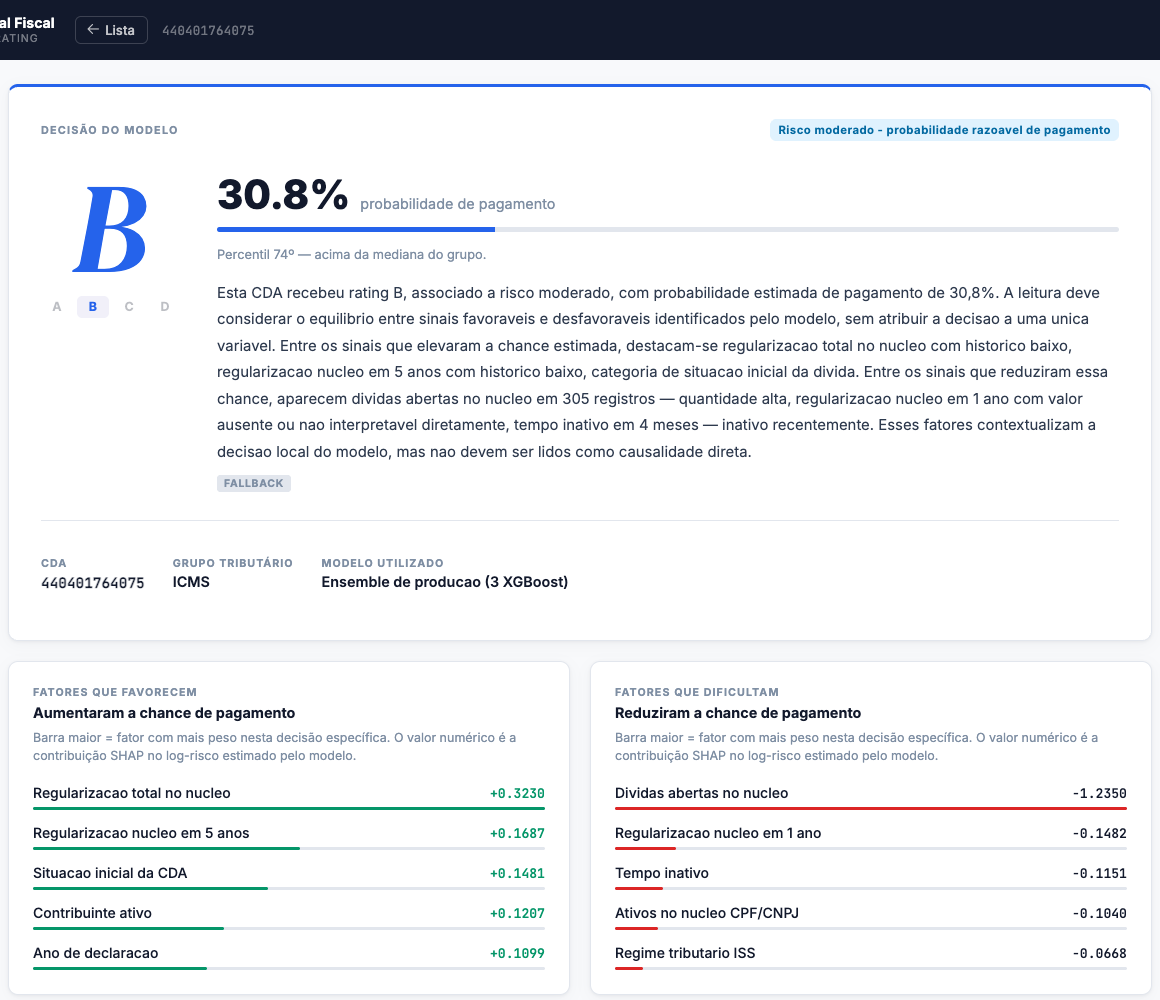
\includegraphics[width=\textwidth]{figuras/app_decisao.png}
    \caption[Ficha de auditoria: decisão do modelo e principais fatores]{Parte superior da ficha de auditoria de uma CDA sintética do ICMS classificada como B. O quadro superior apresenta a decisão do modelo e o texto explicativo; os dois quadros inferiores listam os fatores que aumentaram e os que reduziram a chance de pagamento, com a contribuição SHAP de cada um na escala de \textit{log-odds}. Captura de tela produzida pelos autores.}
    \label{fig:app_decisao}
\end{figure}

A parte inferior da ficha (Figura \ref{fig:app_graficos}) traz o gráfico das contribuições SHAP da CDA, um histograma que situa sua probabilidade na distribuição do \textit{setup} e uma tabela com todas as variáveis, o valor de cada uma na CDA e a intensidade de sua contribuição. A interface avisa, junto às contribuições, que elas medem o peso de cada variável na saída do modelo e não implicam causalidade.

\begin{figure}[H]
    \centering
    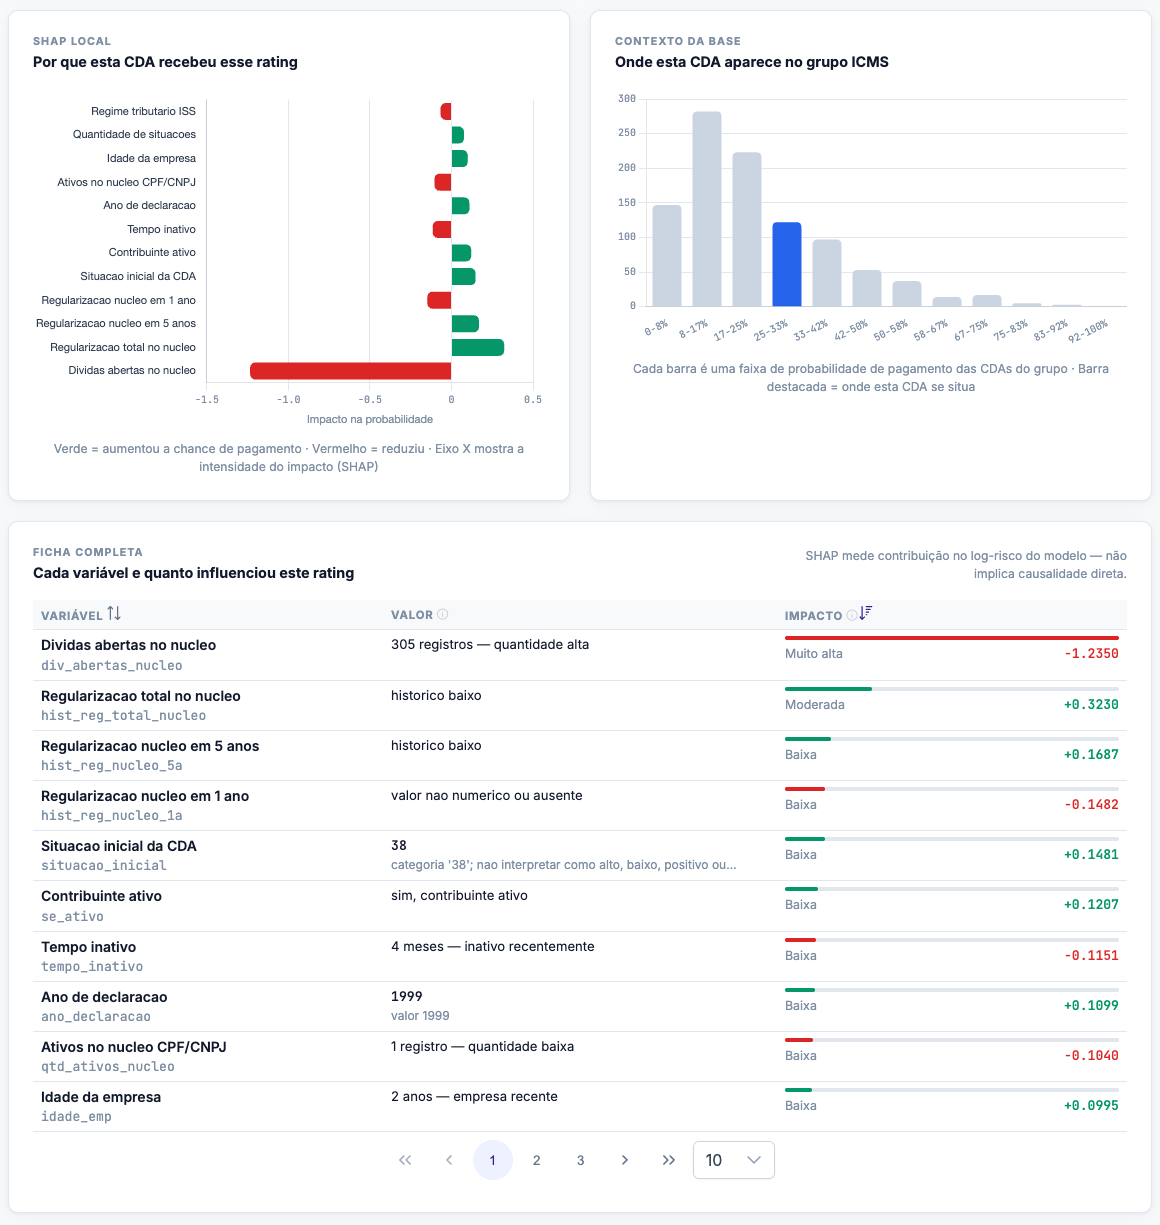
\includegraphics[width=\textwidth]{figuras/app_graficos.png}
    \caption[Ficha de auditoria: gráficos e ficha completa]{Parte inferior da ficha de auditoria da mesma CDA. À esquerda, as contribuições SHAP por variável (verde: aumentou a chance de pagamento; vermelho: reduziu); à direita, a posição da CDA na distribuição de probabilidades do \textit{setup}; abaixo, a ficha completa, com o valor de cada variável e sua contribuição. Captura de tela produzida pelos autores.}
    \label{fig:app_graficos}
\end{figure}

A aplicação apresenta apenas as explicações SHAP. O LIME não foi incorporado porque, por ser estocástico, exibiria explicações diferentes a cada consulta da mesma CDA, o que é inadequado para a fundamentação de um ato administrativo. A aplicação não foi avaliada com auditores fiscais; sua contribuição, neste trabalho, é demonstrar a viabilidade de levar a explicação local ao ponto de uso, e a avaliação com usuários é indicada como trabalho futuro.
